% !TeX spellcheck = pt_PT
% !TeX encoding = UTF-8
\documentclass[a4paper,titlepage]{article}

\usepackage[utf8]{inputenc}
\usepackage[portuguese]{babel}
\usepackage{hyperref}
\usepackage{listingsutf8}
\usepackage{float}
\usepackage{color}
\usepackage[usenames,dvipsnames]{xcolor}
\usepackage{graphicx}
% \usepackage{indentfirst}
\usepackage{epstopdf}
\usepackage{eurosym}
\usepackage{tabularx}
\usepackage{svg}
\usepackage{fancyhdr}
\usepackage{pdfpages}

% Uma forma de usar caracteres especiais nos ficheiros de código-fonte.
\lstset{literate=%
 {á}{{\'a}}1 {é}{{\'e}}1 {í}{{\'i}}1 {ó}{{\'o}}1 {ú}{{\'u}}1
   {Á}{{\'A}}1 {É}{{\'E}}1 {Í}{{\'I}}1 {Ó}{{\'O}}1 {Ú}{{\'U}}1
   {à}{{\`a}}1 {è}{{\'e}}1 {ì}{{\`i}}1 {ò}{{\`o}}1 {ò}{{\`u}}1
   {À}{{\`A}}1 {È}{{\'E}}1 {Ì}{{\`I}}1 {Ò}{{\`O}}1 {Ò}{{\`U}}1
   {ä}{{\"a}}1 {ë}{{\"e}}1 {ï}{{\"i}}1 {ö}{{\"o}}1 {ü}{{\"u}}1
   {Ä}{{\"A}}1 {Ë}{{\"E}}1 {Ï}{{\"I}}1 {Ö}{{\"O}}1 {Ü}{{\"U}}1
   {â}{{\^a}}1 {ê}{{\^e}}1 {î}{{\^i}}1 {ô}{{\^o}}1 {û}{{\^u}}1
   {Â}{{\^A}}1 {Ê}{{\^E}}1 {Î}{{\^I}}1 {Ô}{{\^O}}1 {Û}{{\^U}}1
   {œ}{{\oe}}1 {Œ}{{\OE}}1 {æ}{{\ae}}1 {Æ}{{\AE}}1 {ß}{{\ss}}1
   {ç}{{\c c}}1 {Ç}{{\c C}}1 {ø}{{\o}}1 {å}{{\r a}}1 {Å}{{\r A}}1
   {õ}{{\~{o}}}1
   {ã}{{\~a}}1
   {€}{{\EUR}}1 {£}{{\pounds}}1
}

%\hypersetup{
%    colorlinks = false,
%    hidelinks
%}

\lstdefinelanguage{ios} {
	morekeywords={enable, interface, exit, no, ip, ipv6, network, dhcp, pool, configure, address, shutdown, route, console, terminal, nd, prefix, tunnel, source, destination, secret, line, password, login, banner, motd, hostname, end, vty, mode, gre, transport, input, router, ospf},
	otherkeywords={default-router, excluded-address, domain-lookup, unicast-routing}, % multi-word keywords! :)
	sensitive=true,
	morecomment=[l]{!}
}

\lstdefinestyle{ioscommands} {
  belowcaptionskip=1\baselineskip,
  breaklines=true,
  breakatwhitespace=true,
  xleftmargin=\parindent,
  extendedchars=true,
  language=ios,
  captionpos=b,
  numbersep=5pt,
  basicstyle=\footnotesize,
  keywordstyle=\bfseries\color{blue},
  commentstyle=\itshape\color{CadetBlue},
  identifierstyle=\color{black},
  frame=single,
  tabsize=2
}

\lstdefinestyle{bare} {
  belowcaptionskip=1\baselineskip,
  breaklines=true,
  breakatwhitespace=true,
  xleftmargin=\parindent,
  extendedchars=true,
  language=ios,
  captionpos=b,
  numbersep=5pt,
  basicstyle=\footnotesize,
  keywordstyle=\footnotesize,
  commentstyle=\footnotesize,
  identifierstyle=\footnotesize,
  frame=single
}

\title{PROJECTO DE REDES 2012 / 2013}

\pagestyle{fancy} %estilo fancy

\lhead{}
 
%\lhead{\rightmark} %escrever na esquerda do cabeçalho
 
%\chead{} %escrever no centro do cabeçalho
 
\rhead{Trabalho Prático Nº1} % escrever na direita do cabeçalho
 
\lfoot{Projecto de Redes - 2013/2014} %escrever na esquerda do rodapé
 
\cfoot{} %escrever no centro do rodapé
\rfoot{\thepage} % escrever na direita do rodapé

\author{
	Dário Jorge  nº 17104\\
	Bruno Calças nº 11598\\
}

\date{Março de 2014}

\begin{document}

	\maketitle
	
	\newpage
	
	\tableofcontents
	
	\newpage
	
	\section{Introdução}
		O cálculo do link budget serve para aferir acerca da viabilidade de uma ligação sem fios
	por rádio frequência. Este calculo pode ser decomposto nos passos seguintes:\\
		- Determinar se existe linha de vista, ou seja se o elipsoide de Fresnel de primeira
	ordem está desobstruído. No caso de não haver linha de vista, o link não é viável.\\
	Aumentar o comprimento do mastro de uma das antenas pode ser suficiente para
	que passe a haver linha de vista. Outra solução passa por encontrar um ponto
	intermédio com linha de vista para os pontos a ligar onde se possa instalar um repetidor.\\
		- Determinar o valor do EIRP tendo em conta a potência do transmissor, as perdas
	dos cabos que ligam o emissor à antena externa e o ganho da antena.\\
		- Determinar as perdas em espaço aberto de acordo com a fórmula de Friis.\\
		- Determinar a potência recebida no receptor.\\
		
	\section{Objectivos}
		- Análise de soluções tecnológicas para a implementação de redes wireless;\\
		- Projecto de redes wireless de acordo com as tecnologias consideradas adequadas
	para os requisitos operacionais e para as condicionantes identificadas no terreno;\\
		
	\section{Topologia}
			\begin{figure}[H]
									\centering
									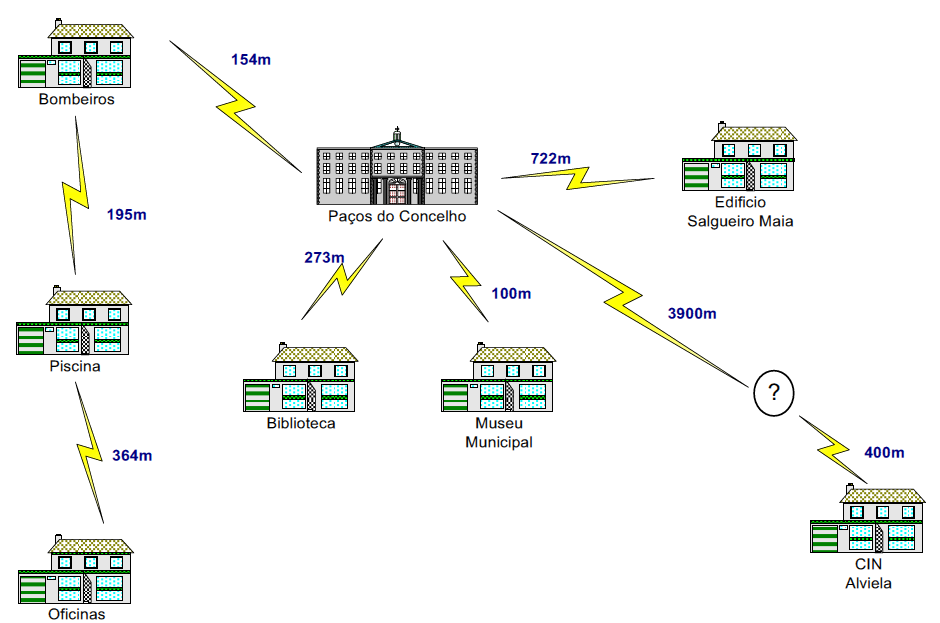
\includegraphics[width=\linewidth]{topologiaTP1.png}
									\caption{Topologia do trabalho}
			\end{figure}
			
	\section{Diagrama De Rede}
		\begin{figure}[H]
											\centering
											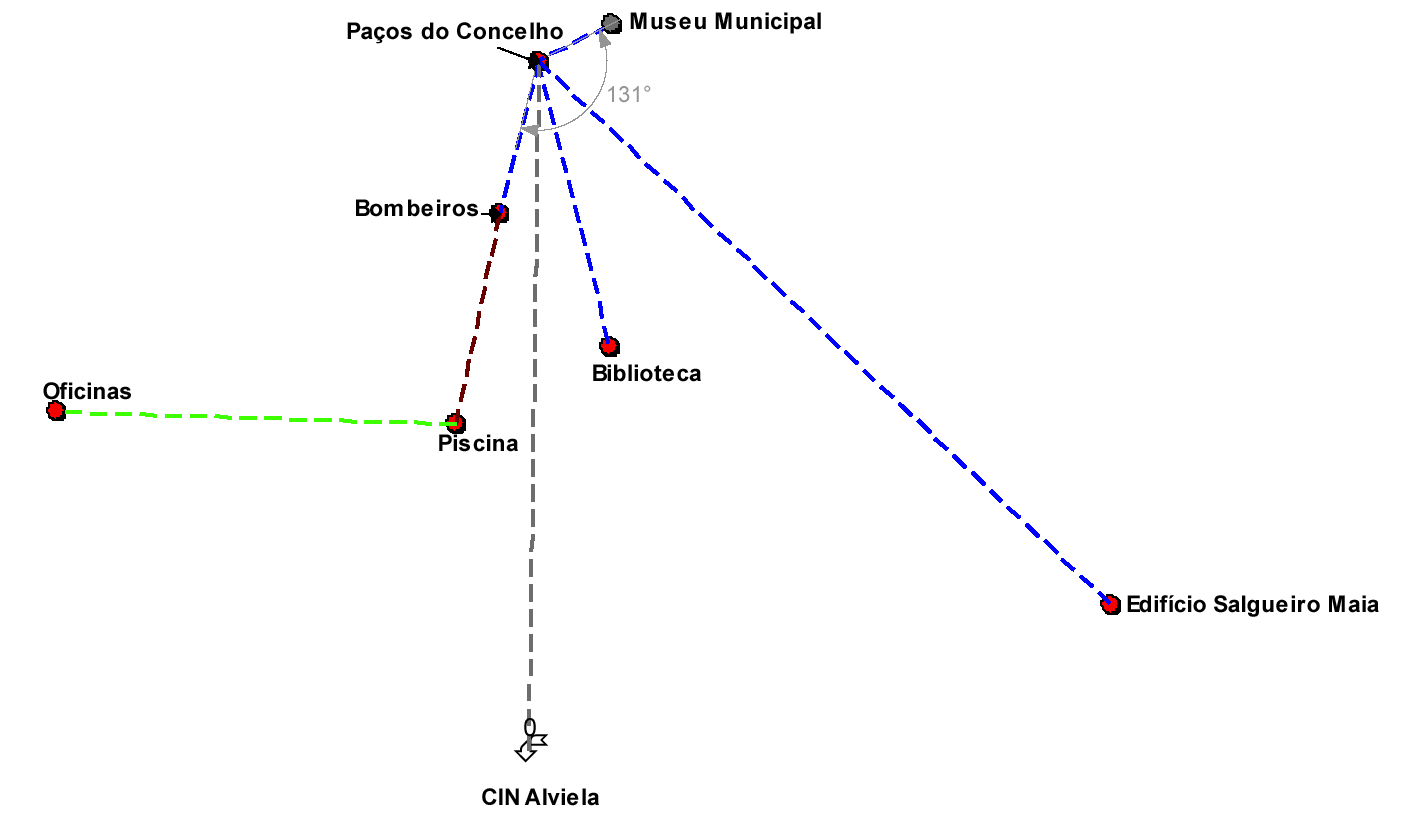
\includegraphics[width=\linewidth]{DiagramaDeRede.png}
											\caption{O diagrama da rede}
		\end{figure}
	\section{Linhas de Vista \& Link Bubget}
		\subsection{Linhas de Vista}
		A primeira parte do trabalho foi determinar se existe linha de vista, ou seja se o elipsoide de Fresnel de primeira ordem está desobstruído. No caso de não haver linha de vista, o link budget não é viável. E uma das soluções passa por elevar as antenas ou por desobstruir o caminho entre as antenas.\\
			
		
		
		\subsection{Link Bubget}
		
		A segunda parte do trabalho passa por determina as variáveis do link budget é o EIRP,ERS e LP(perdas em espaço aberto) o link não é viável se não estiver entre 6 a 10 db se não houver linha de vista nem se tenta calcular o link budget.\\
			\subsubsection{Cálculo do link budget (balanço de potências)}
			– Pode-se dividir o balanço de potência de uma ligação em 3
		partes:\\
				1 - Potência transmitida efectiva: potência transmitida [dbm] +
		ganho antena [dBi] + perdas do cabo e conector [dB]\\
				2 - Perdas na propagação: perdas em espaço livre [dB]\\
				3 - Sensibilidade efectiva do receptor: ganho da antena [dbi] +
		perdas do cabo e conector [dB] + sensibilidade [dBm]\\
		%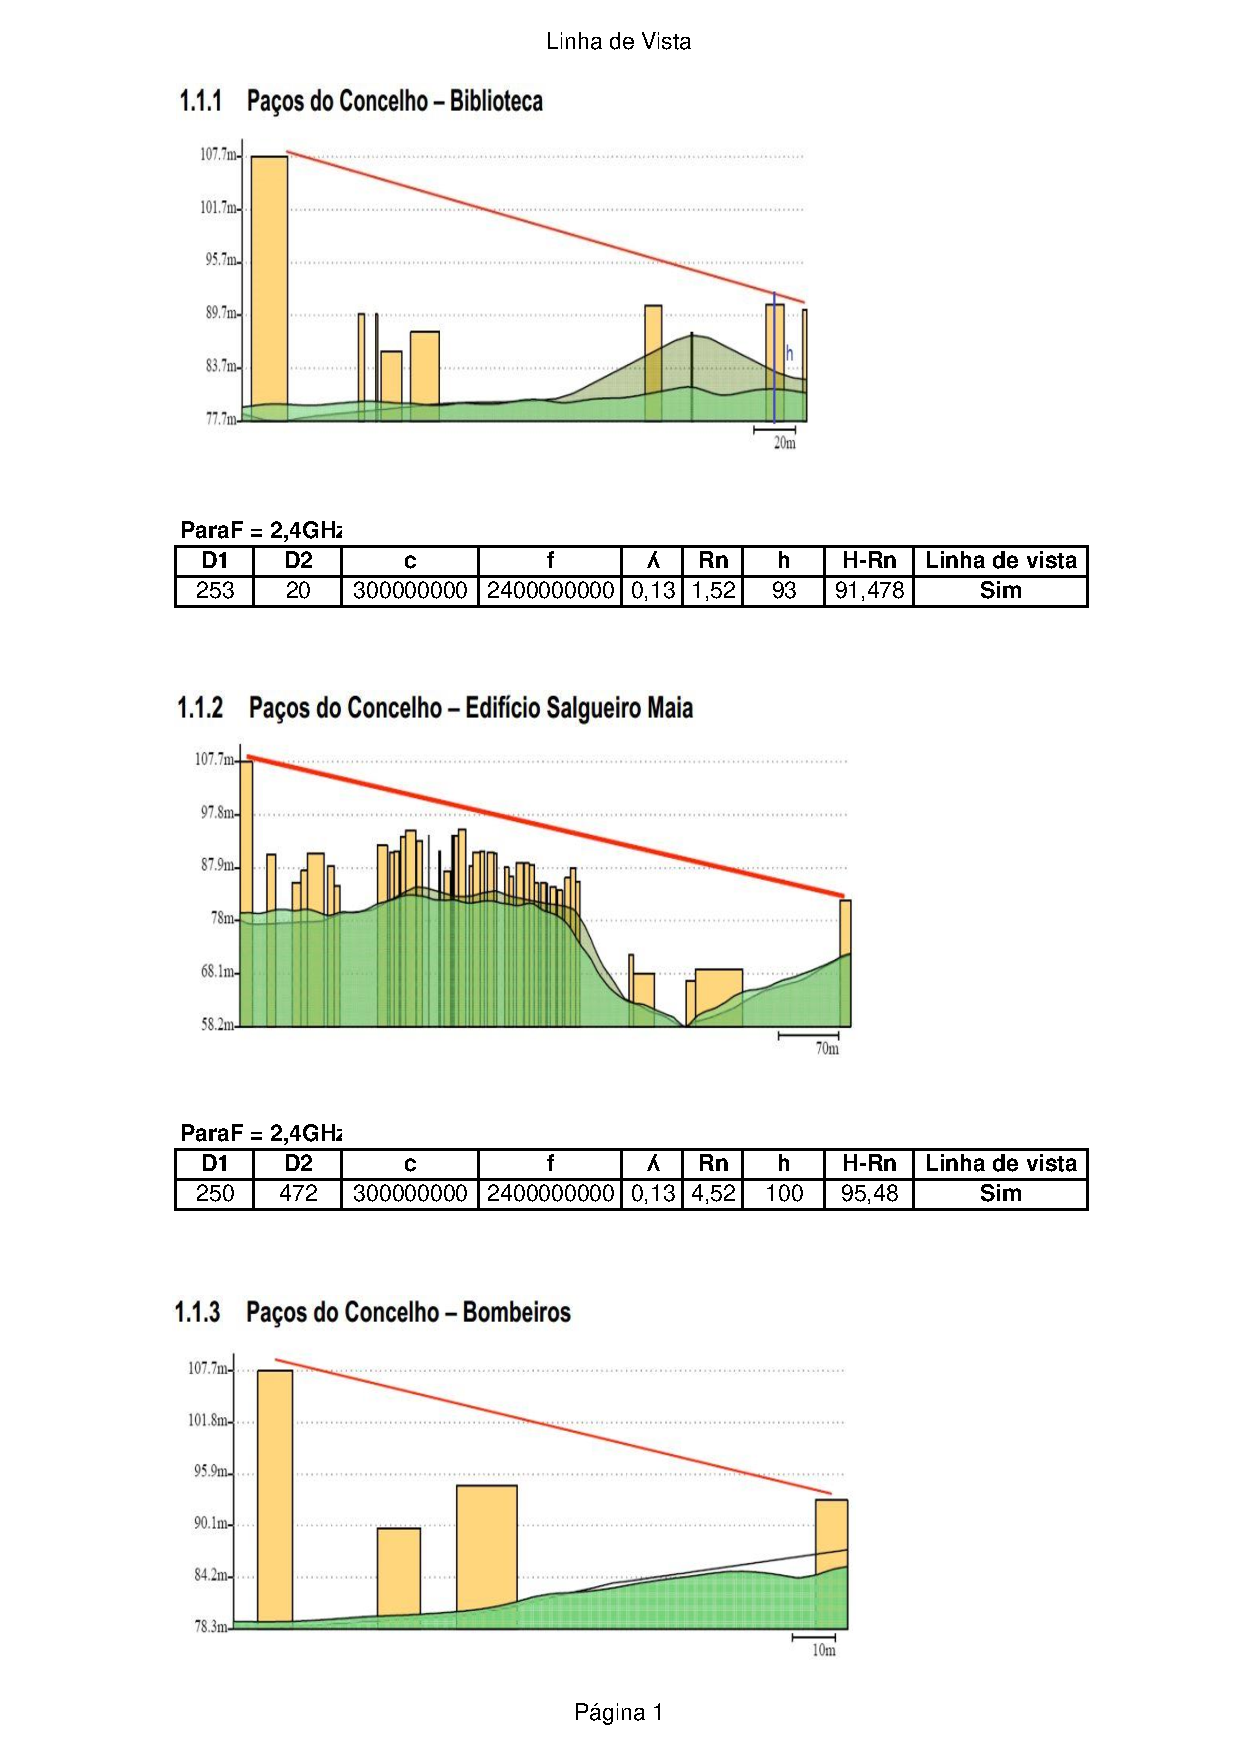
\includepdf[pages=1-3]{calc.pdf} % server para carregar o pdf para o pdf que estás a criar, ou seja serve para caso se precise de um doc do tipo word, exel, etc... passa-se para pdf e zaz!
		\section{Resolução Linhas de Vista}
		
		\begin{figure}[H]
											\centering
											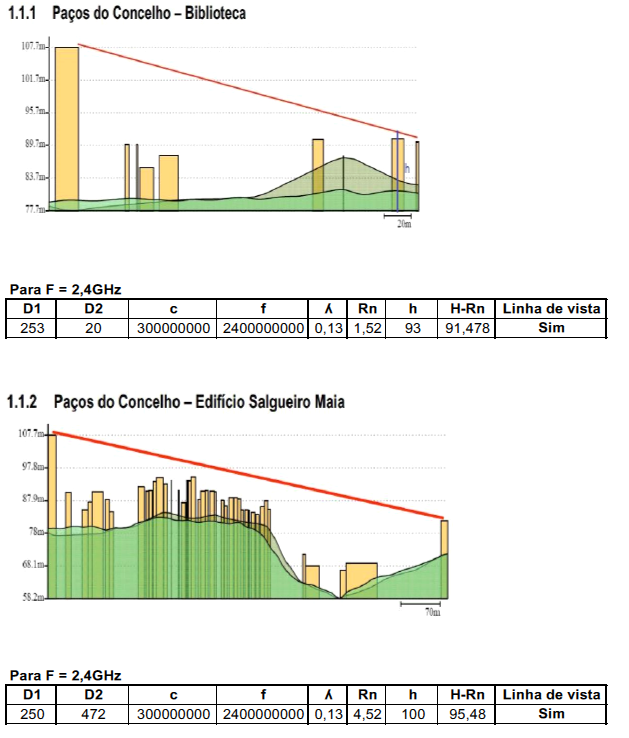
\includegraphics[width=\linewidth]{Img1.png}
		\end{figure}
		\begin{figure}[H]
											\centering
											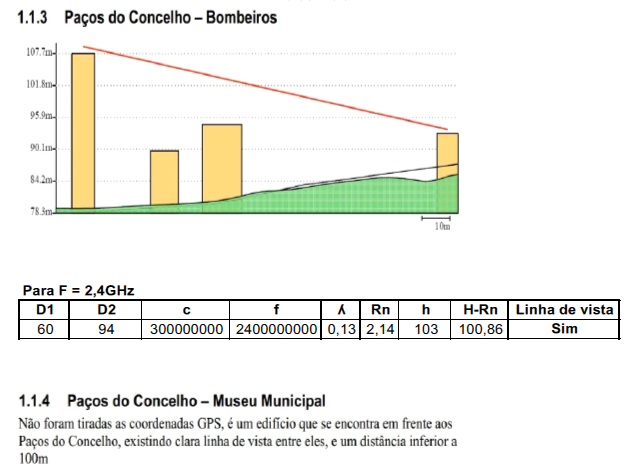
\includegraphics[width=\linewidth]{Img2.png}
		\end{figure}
		\begin{figure}[H]
											\centering
											\includegraphics[width=\linewidth]{Img3.png}
		\end{figure}
		\begin{figure}[H]
											\centering
											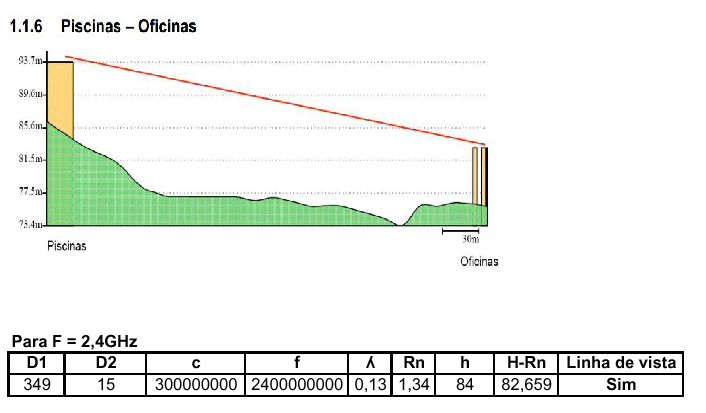
\includegraphics[width=\linewidth]{Img4.png}
		\end{figure}
		\begin{figure}[H]
											\centering
											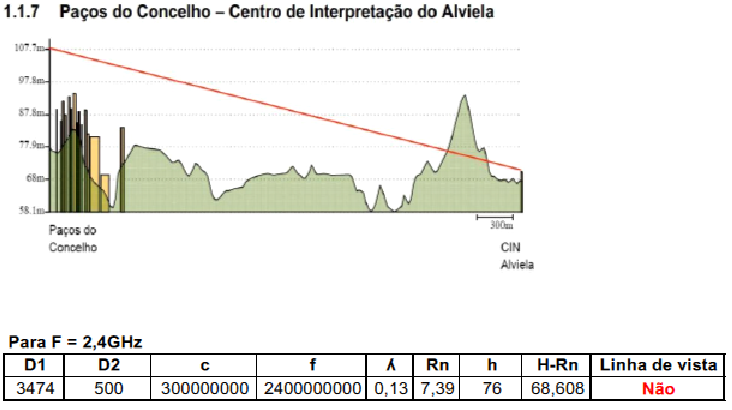
\includegraphics[width=\linewidth]{IMG5_1.png}
		\end{figure}
		\begin{figure}[H]
											\centering
											\includegraphics[width=\linewidth]{Img5_2.png}
		\end{figure}
		\begin{figure}[H]
											\centering
											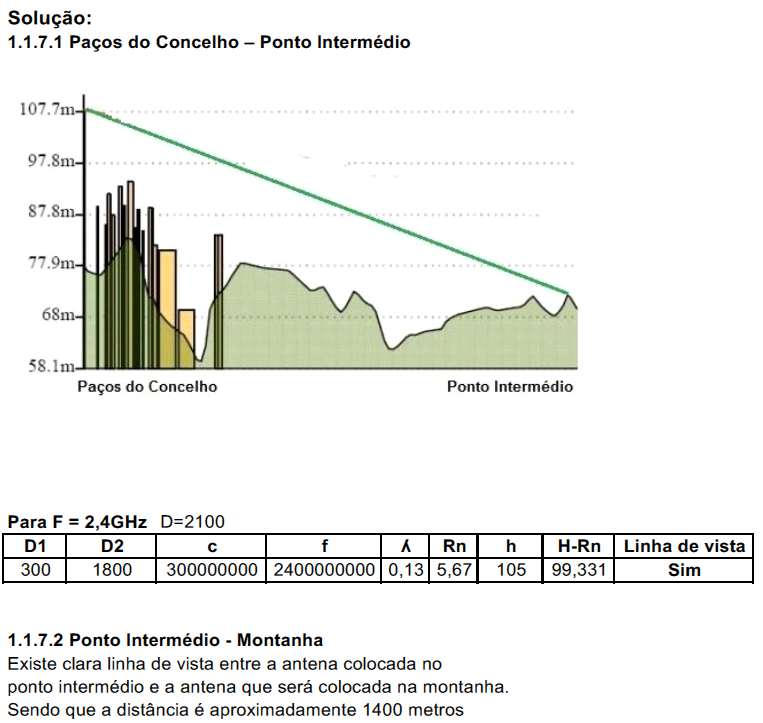
\includegraphics[width=\linewidth]{Img6.png}
		\end{figure}
		\section{Resolução Link Budget}
		\begin{figure}[H]
											\centering
											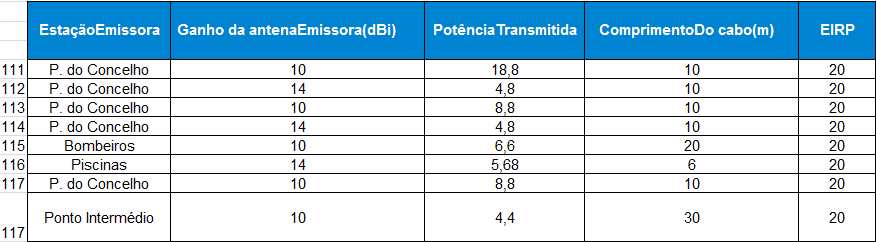
\includegraphics[width=\linewidth]{TAB1.png}
		\end{figure}
		\begin{figure}[H]
											\centering
											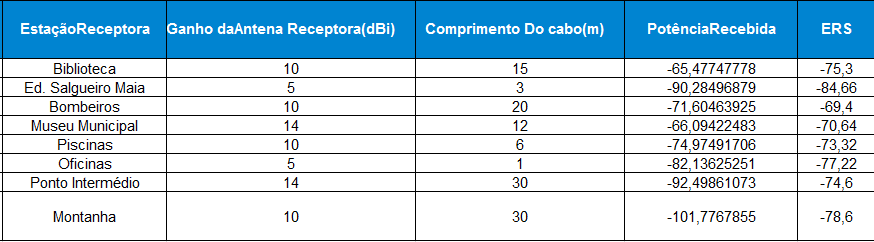
\includegraphics[width=\linewidth]{TAB2.png}
		\end{figure}
		\begin{figure}[H]
											\centering
											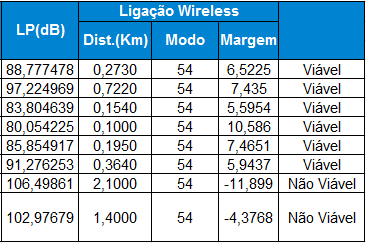
\includegraphics[width=\linewidth]{TAB3.png}
		\end{figure}
		\begin{figure}[H]
											\centering
											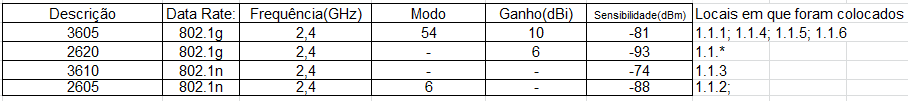
\includegraphics[width=\linewidth]{TABAP.png}
											\caption{Tabela do AP}
		\end{figure}
		\begin{figure}[H]
											\centering
											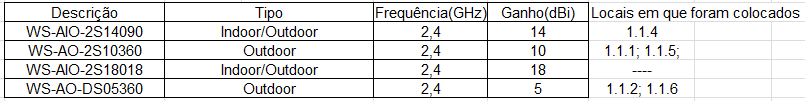
\includegraphics[width=\linewidth]{TABANTEXT.png}
											\caption{Tabela da antena externa}
		\end{figure}
		\section{Glossário}
			\begin{tabular}{|c|c|c|c|}
			\hline D1 & Distância do inicio até ao 1º obstáculo & D2 & Distância do obstáculo até ao fim\\ 
			\hline f & frequência & Rn & O raio da elipsóide de fresnel no ponto \\ 
			\hline H-Rn & A subtração entre a altura e o raio no ponto & c & velocidade da luz \\ 
			\hline h & altura & N/A & N/A \\ 
			\hline 
		\end{tabular} 
\end{document}
